\documentclass[11pt,a4paper]{article}
\usepackage{graphicx}
\usepackage{amssymb}
\usepackage{float}
\usepackage{amsmath}
\DeclareGraphicsExtensions{.pdf,.png,.jpg}

\begin{document}

\title{CS6690: Pattern Recognition Assignment \#2}
\author{Group 3: Akshay \& Suthirth}
\maketitle

\newpage

\section{Bayesian Classifiers}
According to Bayes Theorem, for a dataset x with classes $\omega_i$, \\
Probability of a datapoint belonging to class $\omega_i$ is defined as: \\
\begin{equation}
P(\omega_i | x) = \frac{(P(x|\omega_i)P((\omega_i))}{P(x)}
\end{equation}
\\ 

\begin{itemize}

	\item Here, $P(x|\omega_i)$ is known as the class likelihood. 
\\ To estimate this value, we require the distribution of $\omega_i$.
Based on the central limit theorem, we can assume that this would be Gaussian distribution for large datasets. 

	\item The value $P(\omega_i)$ is the class prior and is calculated using:
		\begin{equation}
		P(\omega_i) = N_i / N  
		\end{equation}
	This term becomes irrelevant if the classes have equal probabilities. 

	\item P(x) is termed as 'evidence' and can be calculated as:
	\begin{equation}
	{P(x) = \sum_i P(x | \omega_i)P(\omega_i)}
	\end{equation}
\end{itemize}

\section{Gaussian Likelihood Distribution}
 
 For multi-dimensional data, the Gaussian Distribution is:   
 \begin{equation}
 P(x;\mu,\Sigma) = \frac{1}{2\pi^{k/2}|\Sigma|^{1/2}} e^{-(x-\mu)^{T} \Sigma^{-1} (x-\mu)}
 \end{equation}
 
 where
 \begin{itemize}
 	\item $\mu$ is the mean 
 	\item $\Sigma$ is the covariance matrix
 \end{itemize}
 
 The above parameters are calculated for the following cases:
\subsection{Data}
Red - Class 1, Green - Class 2, Blue - Class 3, Cyan - Class 4\\
Black (solid) - 1st Eigenvector\\
Black (dashed) - 2nd Eigenvector\\  
\begin{figure}[H]
		\centering
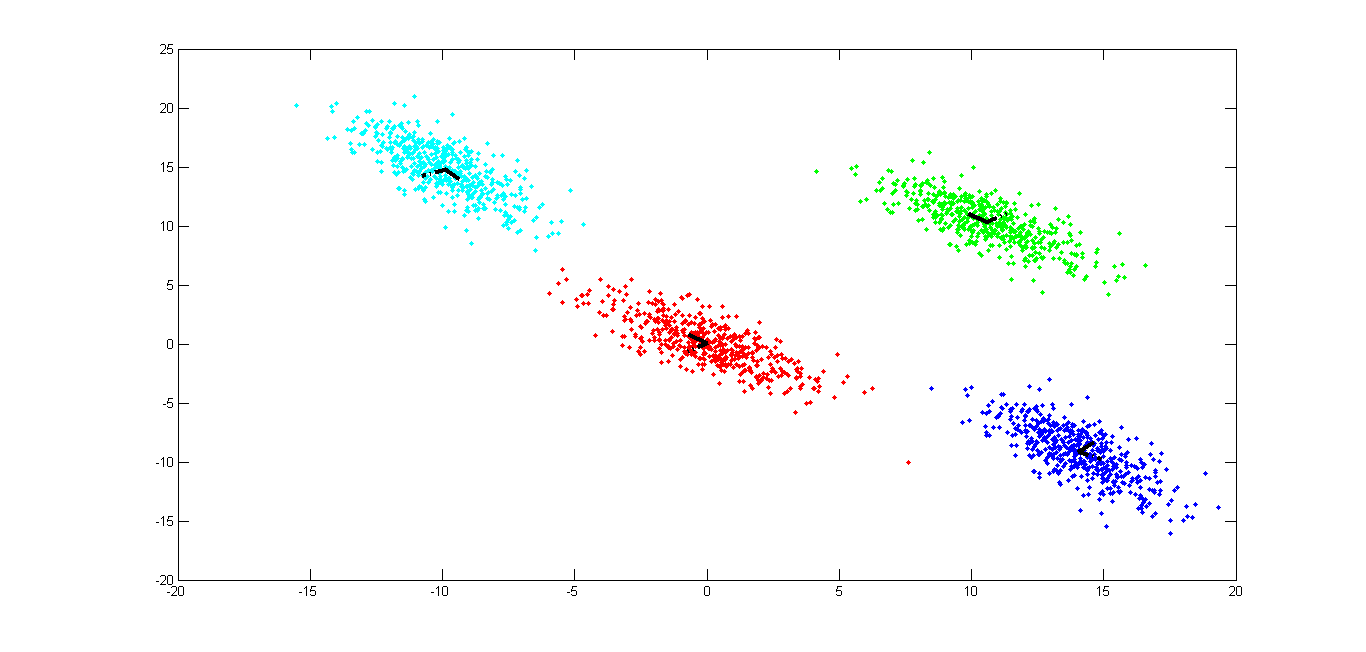
\includegraphics[height=7cm]{Figures/ls_eig.png}
\caption{Linearly Separable Data}
\end{figure}

\begin{figure}[H]
		\centering
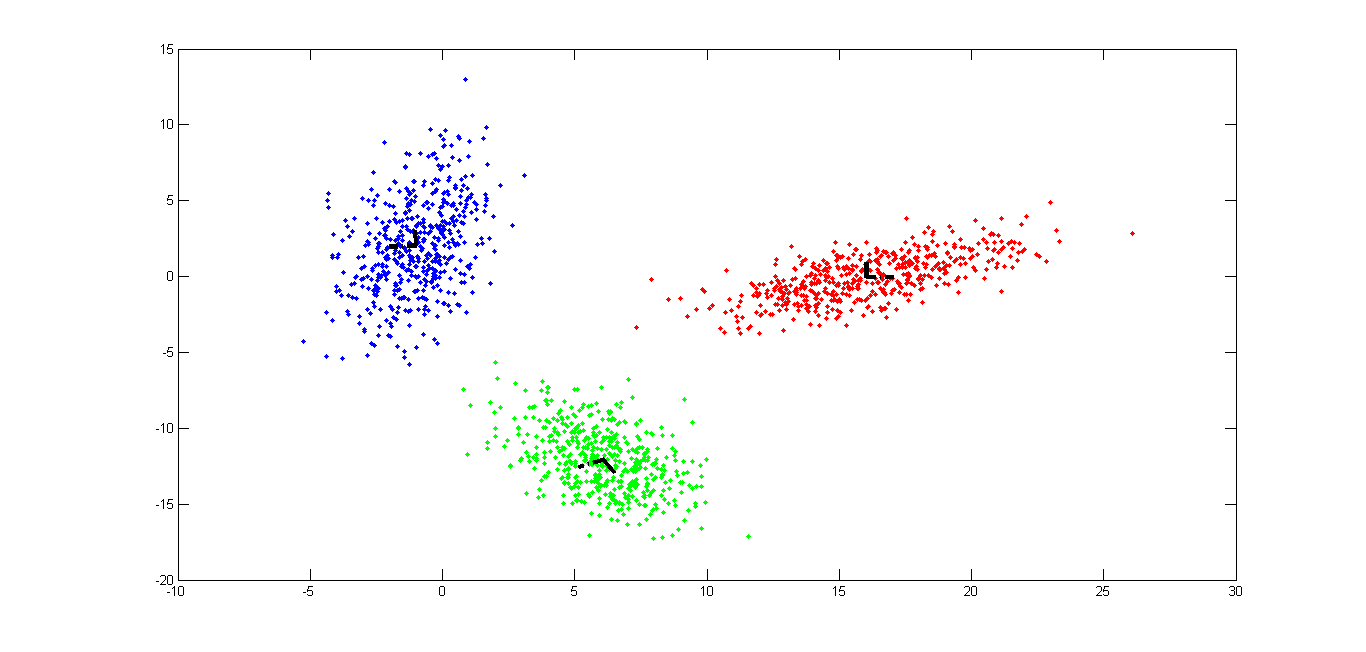
\includegraphics[height=7cm]{Figures/NLS_eig.png}
\caption{Non-linearly Separable Data}
\end{figure}

\clearpage
\begin{figure}[H]
		\centering
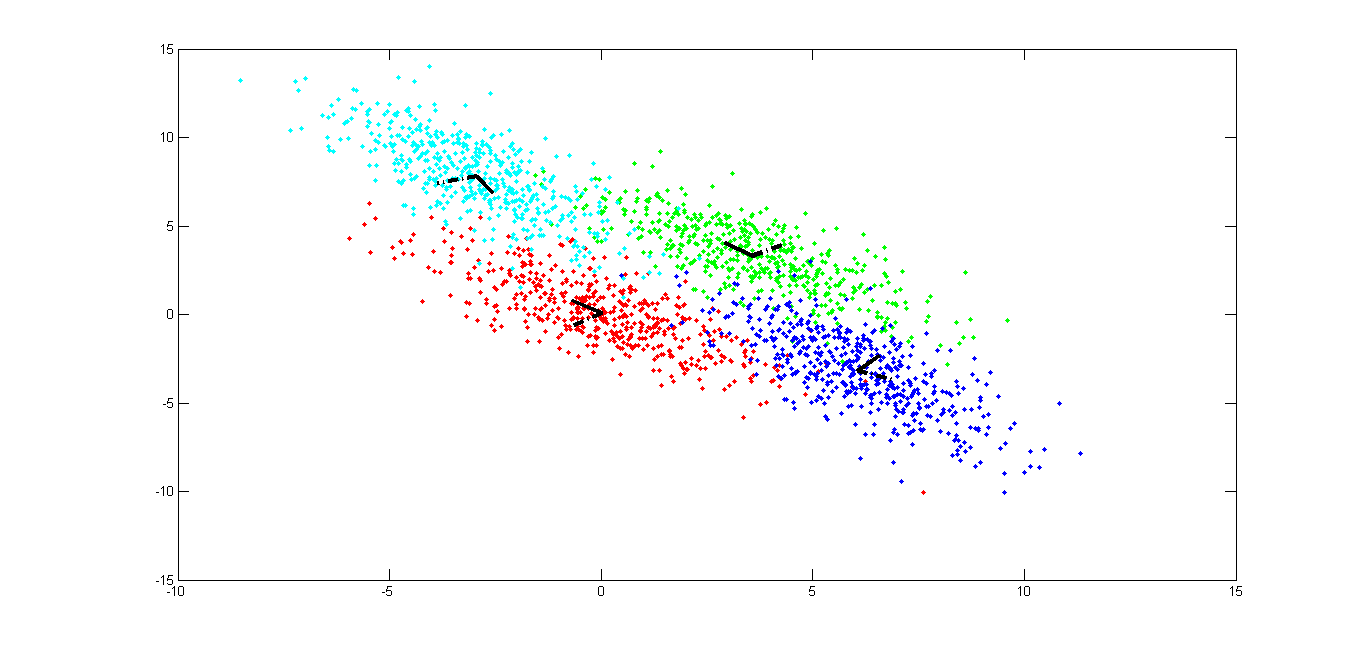
\includegraphics[height=7cm]{Figures/OD_eig.png}
\caption{Overlapping Data}
\end{figure}

\begin{figure}[H]
	\centering
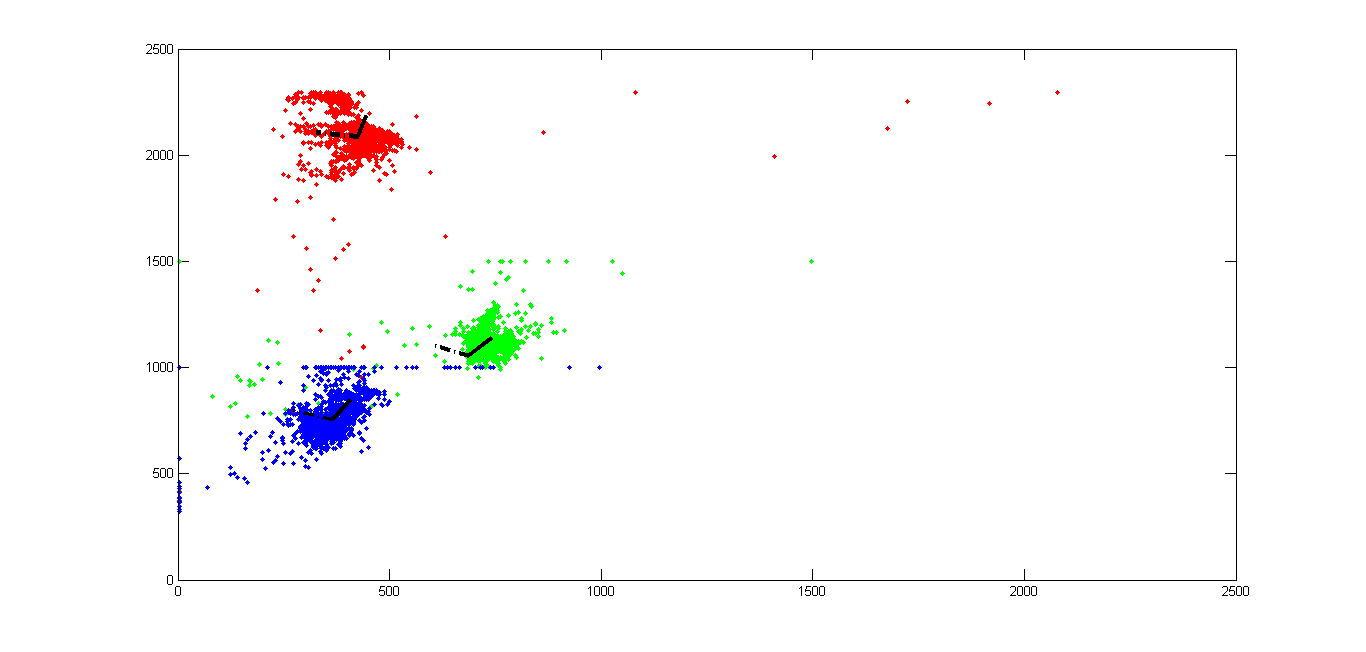
\includegraphics[height=7cm]{Figures/RWD_eig.png}
\caption{Real World Data: Vowel utterance formant frequencies F1 and F2}
\end{figure}

\clearpage
 \subsection{Bayes Classifier with Covariance same for all classes}
\begin{figure}[H]
		\centering
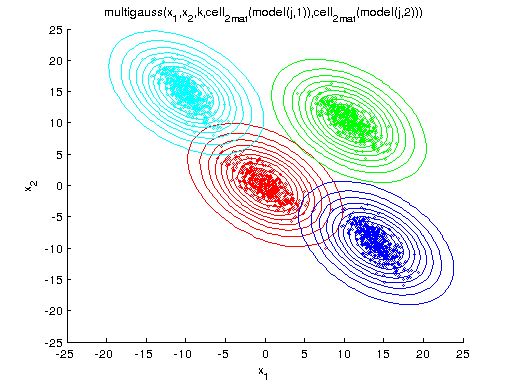
\includegraphics[height=7cm]{Figures/contour_1.png}
\end{figure}
For a bayesian classifier with a common covariance matrix, we combine the matrices by taking the mean of all the class covariance matrices. Geometrically this will result in a linear rotation of the contours, while at the same time, scaling the axes of the contours. 
 \subsection{Bayes Classifier with Covariance different for all classes}
 \begin{figure}[H]
		\centering
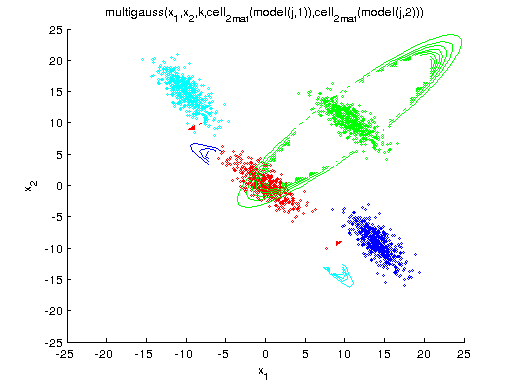
\includegraphics[height=7cm]{Figures/contour_2.png}
\end{figure}
In this case, we take the class matrices and find out standard covariance to get the covariance matrix of each class. This acts as the C in our formula
 \subsection{Naive Bayes Classifier with C = $\sigma^2*I$}
 \begin{figure}[H]
		\centering
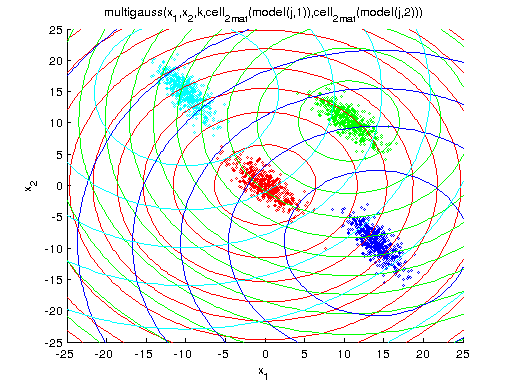
\includegraphics[height=7cm]{Figures/contour_3.png}
\end{figure}
To get one single value of $\sigma$, we use a weighted mean for all the features of each class and come up with a common $\sigma_iI$ matrix; We then take a weighted mean of these matrices to come up with one single $\sigma^2I$ matrix
 \subsection{Naive Bayes Classifier with C same for all classes}
  \begin{figure}[H]
		\centering
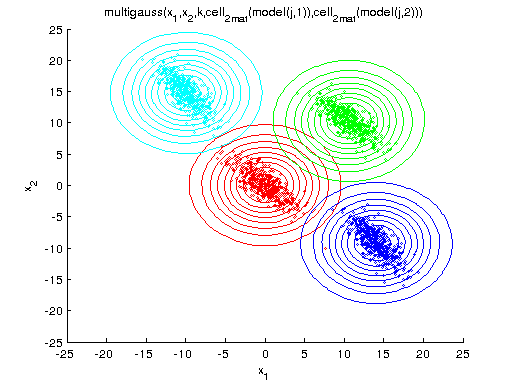
\includegraphics[height=7cm]{Figures/contour_4.png}
\end{figure}
We follow the same principle as the non-naive case, but with features being independent of each other, thus setting off diagonal elements to 0
 \subsection{Naive Bayes Classifier with C different for all classes} 
  \begin{figure}[H]
		\centering
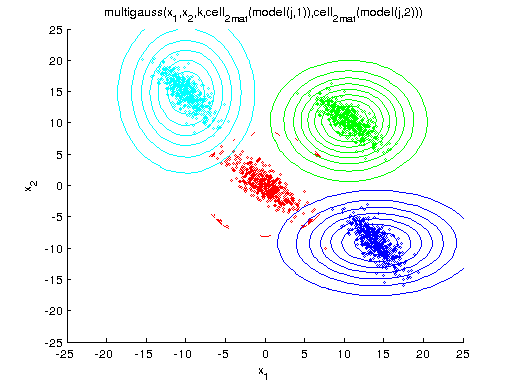
\includegraphics[height=7cm]{Figures/contour_5.png}
\end{figure}
We follow the same principle as the non-naive case, but with features being independent of each other, thus setting off diagonal elements to 0

\section{Bayes Classification}

If $P(\omega_1 | x) > P(\omega_2 | x)$ then x belongs to class $\omega_1$
\\If $P(\omega_1 | x) < P(\omega_2 | x)$ then x belongs to class $\omega_2$\\

Using equation (1), this can be written as:
 \begin{equation}
 {P(x| \omega_1)P(\omega_1) \gtrless P(x | \omega_2)P(\omega_2)}
 \end{equation}

 The value $x_0$ at which the RHS and LHS is called the threshold value. \\

This classification rules minimizes number of misclassifications. \\ \\ 

Based on this classification, the following quantities can be defined:\\ \\
$True Positive Rate = \frac{\Sigma True Positive}{\Sigma Condition Positive}$ \\ \\ 
$False Positive Rate = \frac{\Sigma False Positive}{\Sigma Condition Negative}$ \\ \\


A plot of these two quantities is known as a DET Curve. 

\clearpage
\section{Experiments}

\subsection{Decision Boundaries}
Following plots describe the decision boundaries for various datasets with different Bayesian classifiers. \\

For every figure,\\
\textbf{Row 1:} Bayes with: (L) Same covariance for all classes, (R) Different covariance for all classes\\
\textbf{Row 2:\textbf{}} Naive Bayes with: (L) $C = \Sigma^2*I$, (R) Same C for all classes\\
\textbf{Row 3:} Naive Bayes with different C for all classes\\

\underline{\textbf{Legends:}}\\
Red - Class 1\\
Green - Class 2\\
Blue - Class 3\\
Cyan - Class 4\\
White - $\mu_1 - \mu_2, \mu_3, \mu_4$\\
Yellow - Decision Boundary b/w Class 1 and 2 \\
Magenta - Decision Boundary b/w Class 1 and 3 \\
Cyan (line) - Decision Boundary b/2 Class 1 and 4 

\begin{figure}[H]
	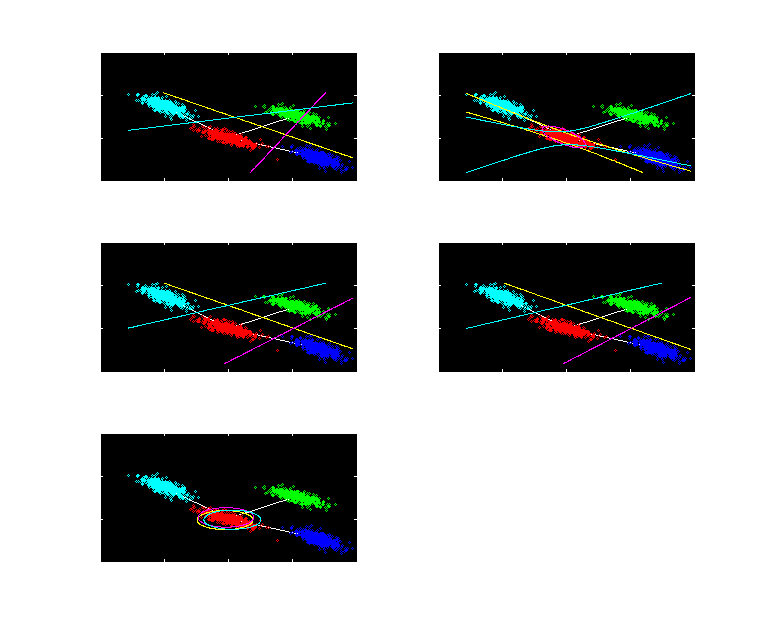
\includegraphics[height=12cm]{Figures/LS_DB.png}
	\caption{Decision Boundary for Dataset 1}
\end{figure}

\begin{figure}[H]
	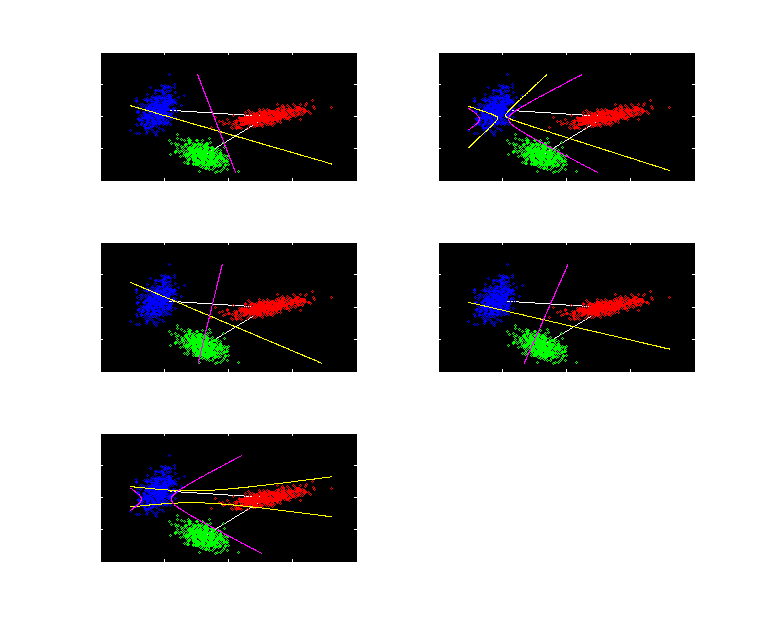
\includegraphics[height=12cm]{Figures/NLS_DB.png}
	\caption{Decision Boundary for Dataset 2}
\end{figure}

\begin{figure}[H]
	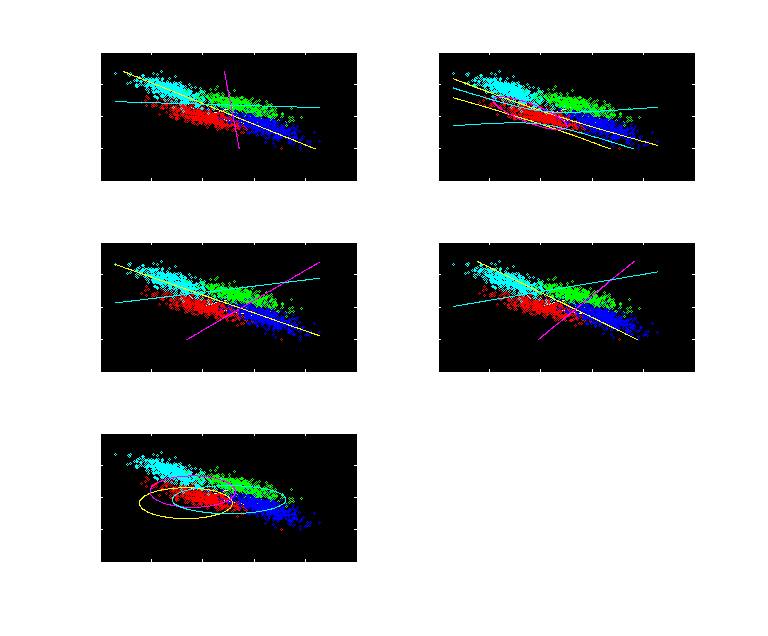
\includegraphics[height=12cm]{Figures/OD_DB.png}
	\caption{Decision Boundary for Dataset 3}
\end{figure}

\begin{figure}[H]
	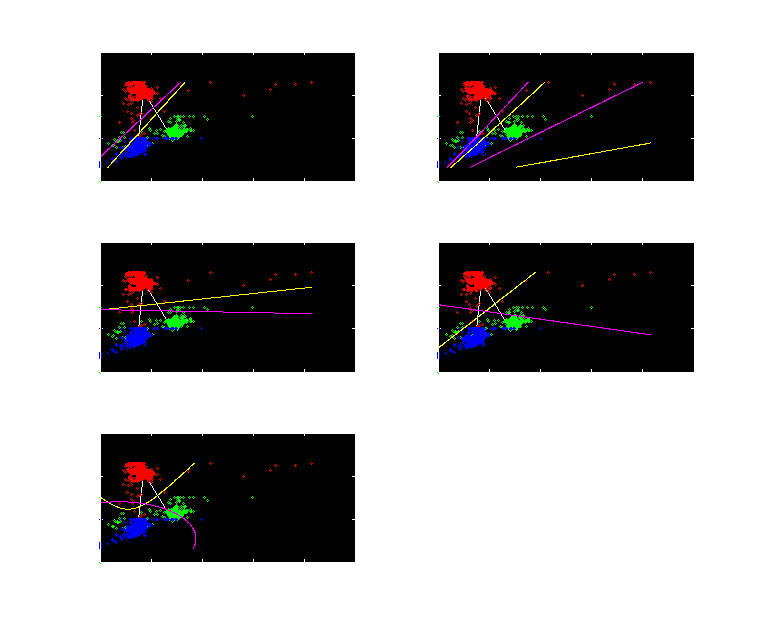
\includegraphics[height=12cm]{Figures/RWD_DB.png}
	\caption{Decision Boundary for Dataset 4}
\end{figure}


\subsection{DET Curves}
\begin{figure}[H]
		\centering
	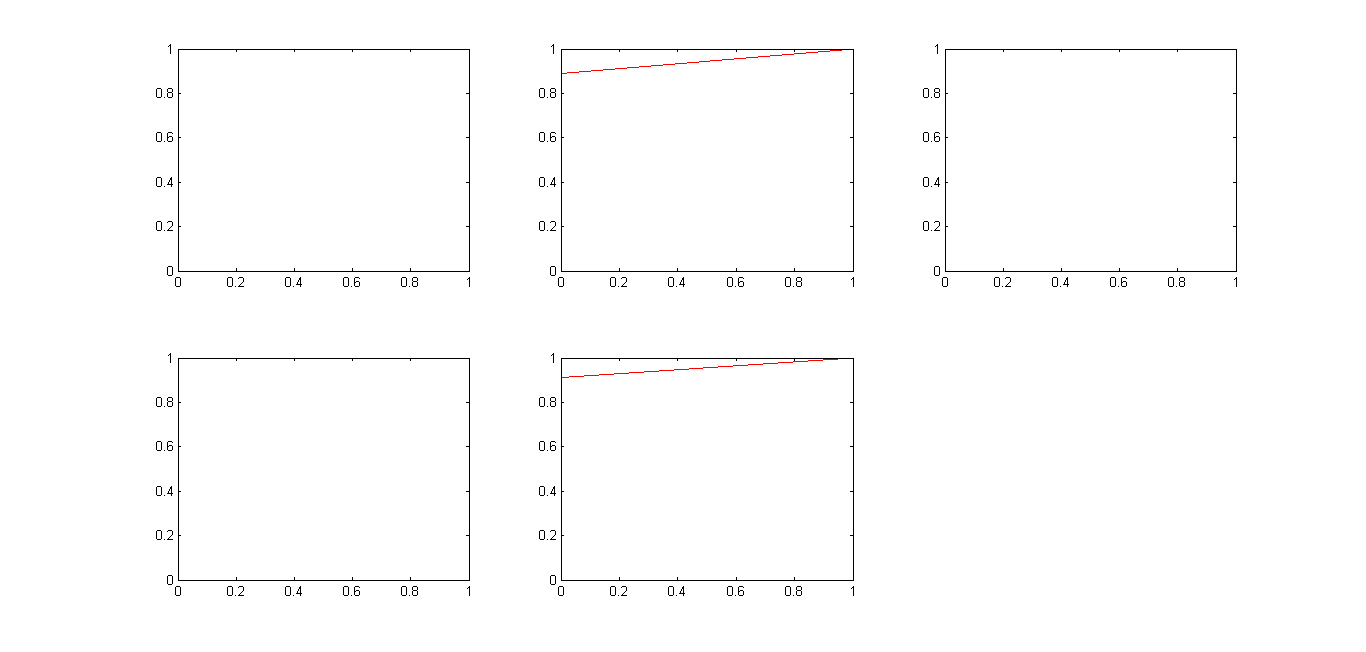
\includegraphics[height=7cm]{DET/1.png}
	\caption{DET Curves for Linearly Separable Data}
\end{figure}

\begin{figure}[H]
		\centering
	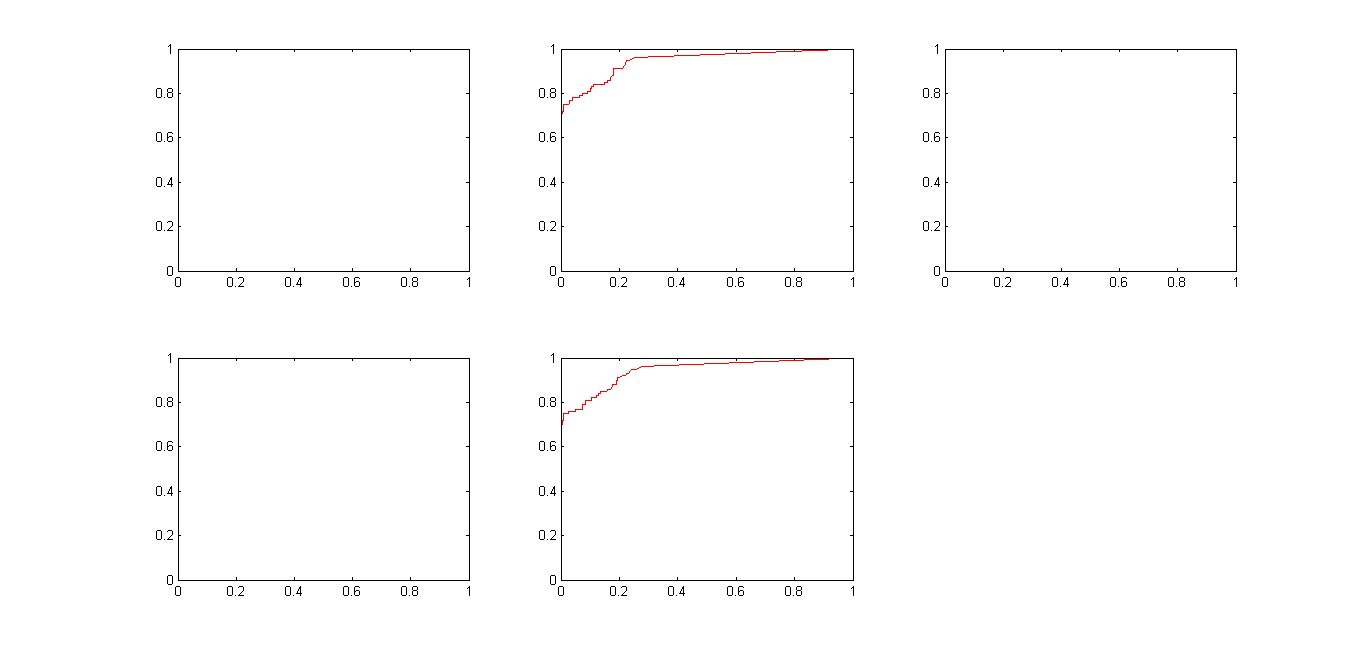
\includegraphics[height=7cm]{DET/2.png}
	\caption{DET Curves for Non-linearly Separable Data}
\end{figure}

\begin{figure}[H]
		\centering
	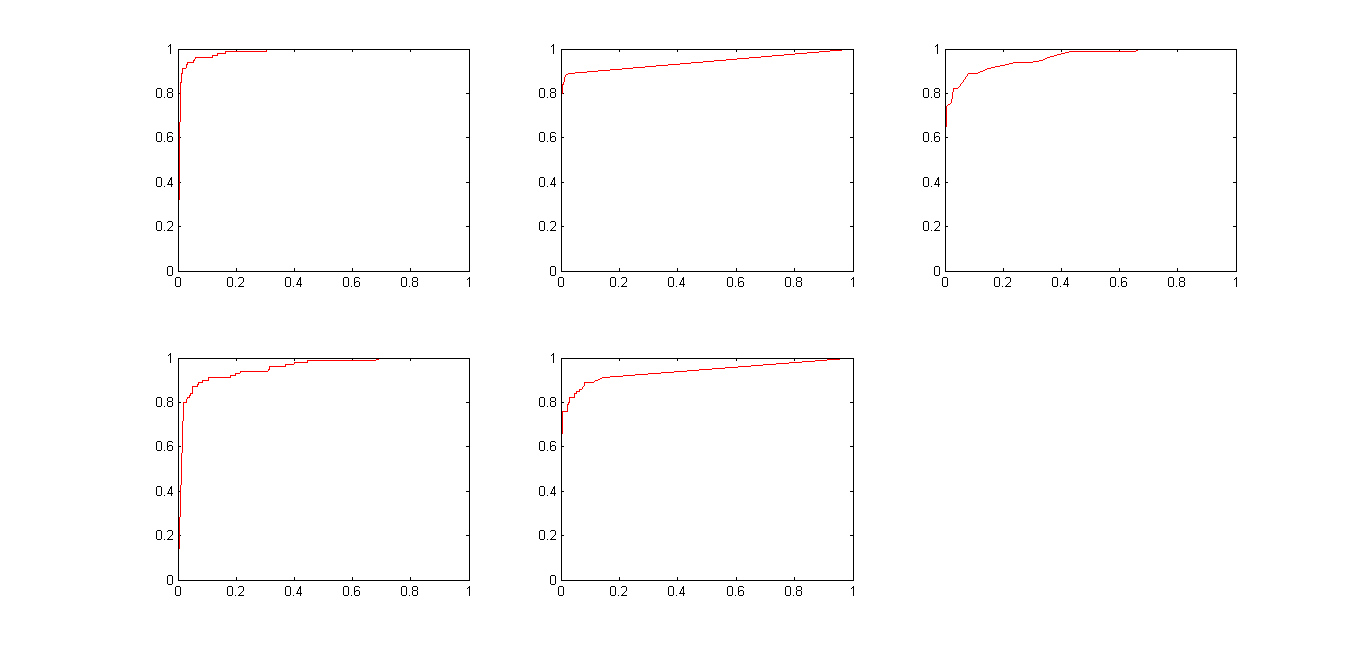
\includegraphics[height=7cm]{DET/3.png}
	\caption{DET Curves for Overlapping Data}
\end{figure}

%\begin{figure}[H]
%		\centering
%	\includegraphics[height=7cm]{DET/4.png}
%	\caption{DET Curves for Real World Data}
% \end{figure}
\section{Confusion Matrix}

\subsection{Case 1}
$$LS = 
\begin{bmatrix}
100   &  0 &    0 &    0 \\
0  & 100   &  0   &  0 \\
0   &  0 &  100  &   0 \\
0   &  0 &    0 &  100
\end{bmatrix}
$$
$$
OD = 
\begin{bmatrix}

 	91 &    0 &    1 &    2 \\
     0 &   92 &   13 &    1 \\
     3 &    2 &   86 &    0 \\
     6 &    6 &    0 &   97

\end{bmatrix}
$$
\subsection{Case 2}
$$LS = 
\begin{bmatrix}
71   &  0 &    0 &    0 \\
10  & 100   &  0   &  0 \\
8   &  0 &  100  &   0 \\
11   &  0 &    0 &  100
\end{bmatrix}
$$
$$ OD = 
\begin{bmatrix}
	64 &    0 &    0 &    0 \\
    12 &   95 &   13 &    4 \\
    14 &    2 &   87 &    0 \\ 
    10 &    3 &    0 &   96 
\end{bmatrix}   
$$
\subsection{Case 3}
$$LS = \begin{bmatrix}
100   &  0 &    0 &    0 \\
0  & 100   &  0   &  0 \\
0   &  0 &  100  &   0 \\
0   &  0 &    0 &  100
\end{bmatrix}
$$
$$
OD = 
\begin{bmatrix}
	86 &    0 &    1 &    2 \\
     0 &   86 &   14 &    4 \\
     6 &    7 &   85 &    0 \\
     8 &    7 &    0 &   94
\end{bmatrix} 	
$$
\subsection{Case 4}
$$ LS = 
\begin{bmatrix}
100   &  0 &    0 &    0 \\
0  & 100   &  0   &  0 \\
0   &  0 &  100  &   0 \\
0   &  0 &    0 &  100
\end{bmatrix}
$$
$$ OD = 
\begin{bmatrix}

 	86 &    0 &     1  &   4 \\
     0  &  87 &   14   &  2 \\
     6   &  7 &   85   &  0 \\
     8   &  6 &    0   & 94 \\
\end{bmatrix}
$$
\subsection{case 5}
$$
LS = \begin{bmatrix}
84   &  0 &    0 &    0 \\
0  & 100   &  0   &  0 \\
6   &  0 &  100  &   0 \\
10   &  0 &    0 &  100
\end{bmatrix}
$$

$$
OD = \begin{bmatrix}
	66  &   0 &    0 &     0 \\
     2  &  89  &  14  &   4 \\
    14   &  5   & 86   &  0 \\
    18    & 6    & 0    & 96 

\end{bmatrix}
$$
\end{document}